\subsection{A.N.F.I.S.}
Finora abbiamo supposto di conoscere a fondo ogni caratteristica del problema che ci viene posto (ci siamo comportati da “esperti”) , supponiamo adesso invece di essere in presenza del seguente scenario:

\begin{itemize}
  \item E' disponibile una collezione di dati (inputs/outputs) da usare per la modellizzazione della rete.
  \item Le funzioni di appartenenza, ed i loro parametri, non sono state arbitrariamente fissate dall'interpretazione dell'esperto.
  \item Non è presente una struttura predeterminata del modello basata sulle caratteristiche delle variabili del sistema.
\end{itemize}

In uno scenario come questo vengono utilizzate quelle che vengono chiamate reti adattive, ovvero reti multistrato dove ogni nodo esegue una particolare funzione sui segnali ricevuti in ingresso, e dove ognuno di essi può contenere (in linea generale) dei parametri.\\

\vspace{20px}
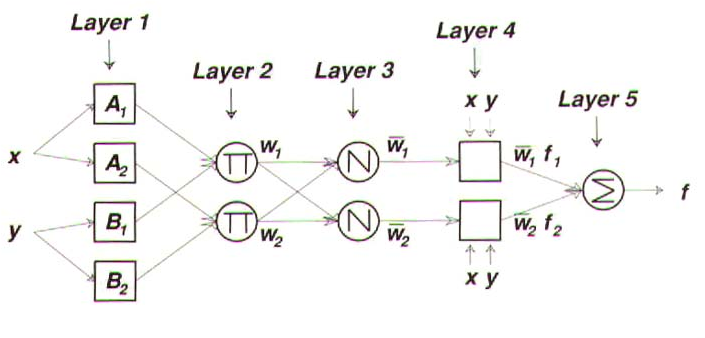
\includegraphics[scale=0.5]{images/anfis/adaptive.png}
\captionof{figure}[One figure]{I nodi quadrati contengono parametri ed eseguono funzioni, gli altri eseguono solo funzioni}
\vspace{20px}

Con il termine A.N.F.I.S. (adaptive network based fuzzy inference system) si indica una classe di reti adattive funzionalmente equivalenti al sistema di inferenza fuzzy; in particolare utilizzando reti di tipo A.N.F.I.S. è possibile costruire una rete del tutto equivalente al sistema di inferenza Takagi-Sugeno-Kang.

Anche in questo caso Matlab mette a disposizione un semplice tool (anfisedit) con il quale è possibile definire una rete A.N.F.I.S.; in questo caso però deve essere già prevista una suddivisione dei dati da presentare al tool, nei casi precedenti invece tale suddivione (training, test e validation) era fatta dai tools in modo automatico.

Nello specifico i dati usati per la fase di training dovrebbero rappresentare in modo completo la realtà così che le funzioni di appartenenza possano essere fissate adeguatamente; anche in questo caso vengono utilizzati due ulteriori files che contengono sia i dati per la fase di checking (analoga alla fase di validation) sia per la fase di tests.

I dati sono stati suddivisi nei tre files a mano (per quanto appena detto) usando le percentuali canoniche: 70\% training, 15\% checking e 15\% tests.

Il tool anfis supporta solamente sistemi di tipo Sugeno, aventi le seguenti condizioni:

\begin{itemize}
  \item Il sistema Sugeno deve essere di grado uno o zero.
  \item Deve presentare una singola uscita ottenuta mediante il metodo di defuzzificazione della media pesata.
  \item Tutte le funzioni di appartenenza dell'uscita devono essere dello stesso tipo e devono essere lineari o costanti.
  \item Diverse regole non possono condividere la stessa funzione di appartenenza di uscita; quindi il numero di funzioni membro delle uscita deve essere uguale al numero di regole.
  \item Possiede peso unitario per ogni regola % FIXME: * Have unity weight for each rule (che minchia vuol dire???)
\end{itemize}

Durante la fase di setup è inoltre richiesto che l'utente specifichi sia quante funzioni di appartenenza andranno usate per gli ingressi ed il tipo (trapezoidali, triangolari etc.), sia il tipo di funzione per l'uscita (lineare o costante).

Bisogna poi indicare il tipo di ottimizzazione usata durante la fase di training ( backpropagation o hybrid), il numero di epoche ed il “training Error Tolerance” per impostare i criteri di stop della fase di allenamento: il processo di training si fermerà dunque quando si raggiunge il massimo numero di epoche o il goal (espresso mediante la error tolerance).


\subsubsection{Ricerca della rete migliore}

Anche in questo caso si è deciso di automatizzare il processo di generazione delle reti; in particolare le variabili su cui la funzione lavora sono principalmente due:
\begin{itemize}
  \item Il numero di funzioni di appartenenza di cui ogni ingresso è composto.
  \item Il numero di epoche della fase di addestramento.
\end{itemize}

Tale funzione (searchBestAnfis) una volta inizializzate le variabili sopra citate, crea la rete e ne misura le performances, ovvero ne calcola l'MSE (mean square error) usando i dati di test.

Se il risultato ottenuto supera il goal (fissato a 20) esce immediatamente; altrimenti controlla se tale MSE è minore di quello della migliore rete trovata fino a questo momento; in caso positivo salva i parametri attuali, altrimenti prosegue semplicemente.

In questo caso sono state modellate tre diverse reti: una per i giorni festivi la cui uscita è la luminosità interna all'edificio e due per i giorni feriali (luminosità ed energia consumata); non è stata creata la rete per l'energia consumata per i giorni festivi in quanto dopo un analisi dei dati si è riscontrato che l'output è praticamente sempre nullo.

Infine le funzioni di appartenenza degli ingressi hanno una forma fissa a “campana” (la forma non è una variabile della funzione), e l'uscita è lineare.


\paragraph{Funzione searchBestAnfis}
La funzione che esegue quanto appena detto è la seguente:

\inputminted[linenos=true,fontsize=\footnotesize]{matlab}{../../src/anfis/functions/searchBestAnfis.m}
\captionof{listing}{src/anfis/functions/searchBestAnfis.m}


\paragraph{Script netanfis}
Lo scopo di tale script è quello di lanciare la funzione sopra enunciata e di resituirne i valori.

\inputminted[linenos=true,fontsize=\footnotesize]{matlab}{../../src/netanfis.m}
\captionof{listing}{src/netanfis.m}

Tale script fa uso della funzione testplot creata appositamente per visualizzare i risultati.


\paragraph{Funzione testplot}
Questa funzione stampa a schermo le uscite di una rete dato un vettore di ingressi.
\inputminted[linenos=true,fontsize=\footnotesize]{matlab}{../../src/anfis/functions/testplot.m}
\captionof{listing}{src/anfis/functions/testplot.m}


\subsubsection{Risultati}

%% FIXME: Qui servirebbero un po piu di figure come ad esempio l'andamento degli errori! L'unica cosa è che avendo svolto questo punto con il tool si ottengono usando anfisedit

Sono sotto riportati i grafici (ottenuti nelle tre reti relativi ai casi di tests) che mostrano le relazioni output/target.\\
\vspace{20px}
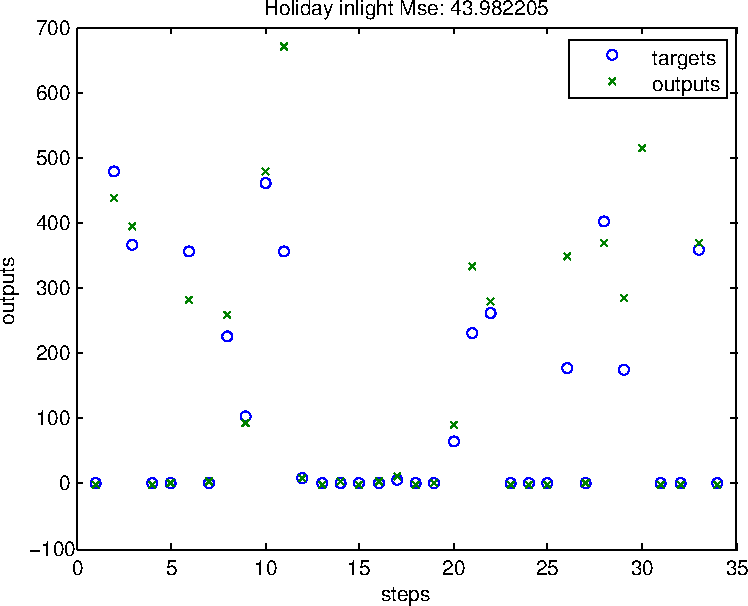
\includegraphics[scale=0.5]{images/anfis/holiday/inlight.pdf}
\captionof{figure}[One figure]{Luce interna nei giorni festivi}
\vspace{20px}

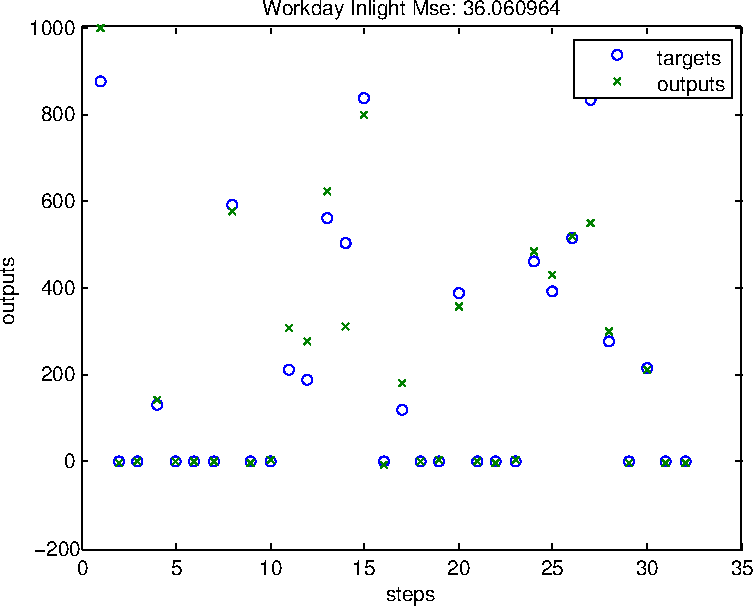
\includegraphics[scale=0.5]{images/anfis/workday/inlight.pdf}
\captionof{figure}[One figure]{Luce interna nei giorni feriali}
\vspace{20px}

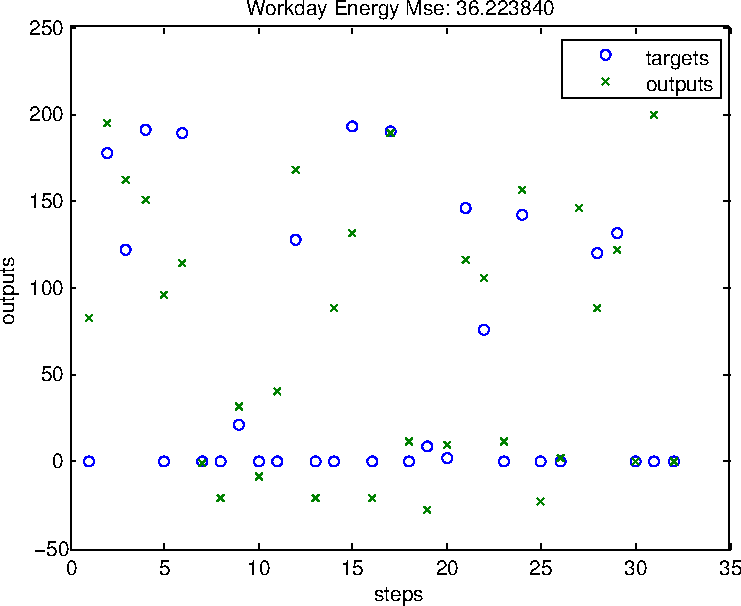
\includegraphics[scale=0.5]{images/anfis/workday/energy.pdf}
\captionof{figure}[One figure]{Energia consumata nei giorni feriali}
\vspace{20px}

La seguente tabella riporta invece i singoli errori (misurati come differenza tra target ed output) delle tre reti:

\begin{table}
  \caption{Risultati}
  \centering
	\begin{tabular}{lll}
		\toprule
    Giorni festivi (Energia) & Giorni feriali (Energia) & Giorni feriali (Luce interna) \\
		\midrule
    -3.4486 & -76.2742 & 31.3233 \\
    -52.2700 & -22.5364 & 16.1849 \\
    25.4036 & -28.7220 & 17.3464 \\
    -101.9807 & 0.9780 & 6.9155 \\
    -100.1104 & 6.3548 & -6.1994 \\
    6.2478 & -1.9842 & 0.7581 \\
    7.5718 & -8.8699 & 6.9155 \\
    -125.6459 & -78.3393 & -2.5798 \\
    -15.8978 & 20.8780 & -2.5798 \\
    -2.2610 & -7.6363 & -42.3179 \\
    -22.4493 & -6.3052 & 54.5844 \\
    -120.6839 & -54.9926 & 23.1033 \\
    2.4897 & 8.1659 & 6.0345 \\
    -1.1282 & -79.8701 & 44.4433 \\
    -4.1744 & -8.6983 & 87.5543 \\
    -9.0550 & -0.1074 & -36.0532 \\
    17.6492 & -44.0539 & 102.1473 \\
    7.8487 & -5.7140 & 3.0584 \\
    2.4897 & -36.5660 & -60.4570 \\
    64.2409 & -8.0969 & -1.3219 \\
    -1.1282 & -39.7330 & 9.3465 \\
    3.0565 & -5.7140 & 0.7581 \\
    0.6982 & -12.0171 & -2.5798 \\
    -4.2594 & 7.7194 & 6.9155 \\
    -46.1005 & -85.7398 & 13.8765 \\
    -35.9813 & -0.1074 & 3.0584 \\
    49.5614 & 29.6689 & -68.8789 \\
    1.3049 & -26.4973 & 4.9651 \\
    -3.2561 & 2.0773 & 64.5088 \\
    -14.3114 & -66.0939 & -15.0161 \\
    -1.1282 & 0.4544 & -6.1994 \\
    -1.1282 & -0.1074 & 0.7581 \\
		\bottomrule
	\end{tabular}
\end{table}

\clearpage
